\langsection[subsection]{Crash Avoidance}{Предотвращение аварий}




\begin{langblock}{0.425}
	\begin{eng}
		
	No matter how careful you are, there will be times when you find yourself in a tight spot. Your chances of getting out safely depend on your ability to react quickly and properly.  Often, a crash occurs because a rider is not prepared or skilled in crash-avoidance maneuvers.
	
	Know when and how to stop or swerve, two skills critical to avoiding a crash. It is not always desirable or possible to stop quickly to avoid an obstacle. Riders must also be able to swerve around an obstacle.  Determining the skill necessary for the situation is important as well.
	
	Studies show that most crash-involved riders:
	
	\begin{description}[noitemsep]
		\item [Underbrake] the front tire and overbrake the rear.
		\item [Did not] separate braking from swerving or did not choose swerving when it was appropriate.
	\end{description}
	
	The following information offers some good advice.
	\end{eng}
	\begin{rus}
		
		Как бы вы ни были осторожны, случится момент, когда вы окажетесь в сложной ситуации. Ваш шанс благополучно выбраться из нее зависит от вашей способности быстро и правильно среагировать. Часто авария происходит из-за того, что мотоциклист не готов или не владеет навыками контр аварийного маневрирования.
		
		Знайте, как и когда остановиться или увернуться "--- эти два навыка имеют решающее значение для предотвращения аварии. Быстрая остановка для избежания препятствия, не всегда целесообразна или осуществима. Мотоциклист должен также уметь объезжать препятствие. Не менее важно уметь определить, что предпочтительнее в какой ситуации.
		
		Исследования показывают, что большинство мотоциклистов, попавших в аварию:
		
		\begin{description}[noitemsep]
		\item [Недостаточно] сильно тормозили передним тормозом и излишне задним.
		\item [Не разделили] торможение и объезд препятствия или выбрали торможение, когда целесообразнее было объехать.
		\end{description}
		Следующая информация содержит несколько полезных советов.
\end{rus}
\end{langblock}

\langsection[subsubsection]{Quick Stops}{Экстренное торможение}

\begin{figure}[htbp]
	\centering
	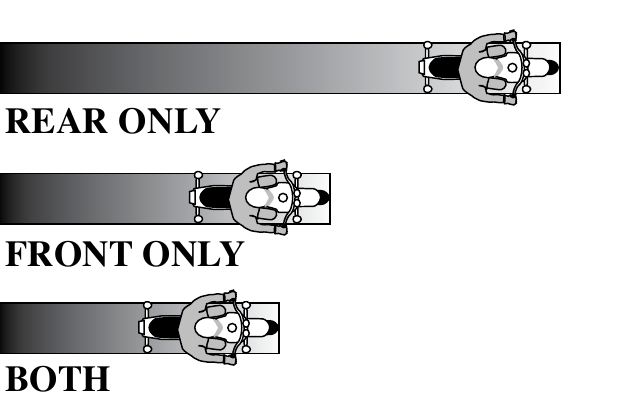
\includegraphics[width=0.45\textwidth, frame]{images/stopping_dist.png}
	\caption{Stopping distance}
	\label{fig:s_dis}
\end{figure}



\begin{langblock}{0.425}
	\begin{eng}
	
	To stop quickly, apply both brakes at the same time. Don't be shy about using the front brake, but don't "grab" it, either. Squeeze the brake lever firmly and progressively. If the front wheel locks, release the front brake immediately then reapply it firmly. At the same time, press down on the rear brake. If you accidentally lock the rear brake on a good traction surface, keep it locked until you have completely stopped.
	
	Even with a locked rear wheel, you can control the motorcycle on a straightaway if it is upright and going in a straight line.
	
	Always use both brakes at the same time to stop. The front brake can provide 70\% or more of the potential stopping power.
	
	If you must stop quickly while turning or riding a curve, the best technique is to straighten the motorcycle upright first and then brake. However, it may not always be possible to straighten the motorcycle and then stop. If you must brake while leaning, apply light brakes and reduce the throttle. As you slow, you can reduce your lean angle and apply more brake pressure until the motorcycle is straight and maximum brake pressure is possible. You should straighten the handlebars in the last few feet of stopping, the motorcycle should then be straight up and in balance.
	\end{eng}
	\begin{rus}
		
		Для быстрой остановки, задействуйте оба тормоза одновременно. Не стесняйтесь использовать передний тормоз, но и не «дергайте» его слишком резко. Сжимайте тормозной рычаг уверенно и плавно. Если переднее колесо заблокировалось, немедленно отпустите передний тормоз, а затем повторите торможение. Одновременно нажимайте и на задний тормоз. Если вы случайно заблокировали задний тормоз на поверхности с хорошим сцеплением, держите его заблокированным до полной остановки!\footnote{Это базовое правило. Если отпустить заблокированный задний тормоз, то мгновенный рывок восстановления сцепления выстреливает зад мотоцикла вверх и в сторону -- это highside, самый травматичный тип падения. На курсах BRC учат как решить эту проблему. Важна оговорка про поверхности с хорошим сцеплением. Чем лучше сцепление тем сильнее и опаснее highside. На песке или гравии негативный эффект ниже.}
		
		Даже с заблокированным задним колесом вы сможете контролировать мотоцикл на прямом участке, если он находится в вертикальном положении и движется по прямой.
		
		Даже для обычных остановок всегда используйте оба тормоза одновременно.\footnote{Привычка всегда тормозить обоими тормозами вырабатывает автоматический навык и позволит в экстренной ситуации задействовать мышечную память.} Передний тормоз может обеспечить где-то 70\% потенциала тормозной силы.
		
		Если вам необходимо экстренно остановиться в повороте или во время маневра, лучший способ "--- сначала выровнять мотоцикл в вертикальное положение, а только потом тормозить. Однако это не всегда возможно. Если вам приходится тормозить в наклоне, сначала плавно закрой газ, затем слегка зажмите тормоза. По мере замедления вы можете уменьшать угол наклона и увеличивать усилие на тормозах, пока мотоцикл не выпрямится и не станет возможным применить максимальное усилие торможения. Вы должны «выпрямить» руль на последнем отрезке торможения; мотоцикл должен находиться в вертикальном положении и равновесие.\footnote{Тут опущен момент про сцепление. Торможение по прямой: сцепление + сброс газа, оба тормоза в пол. Но если байк в наклоне: сначала плавное закрытие газа, затем плавное торможение пока не появится возможность выпрямиться, а уже потом "--- сцепление, тормоза в пол.}
\end{rus}
\end{langblock}






\langsection[subsubsection]{Swerving or Turning Quickly}{Уклонение и маневрирование}



\begin{figure}[htbp]
	\begin{subfigure}{0.45\textwidth}	
		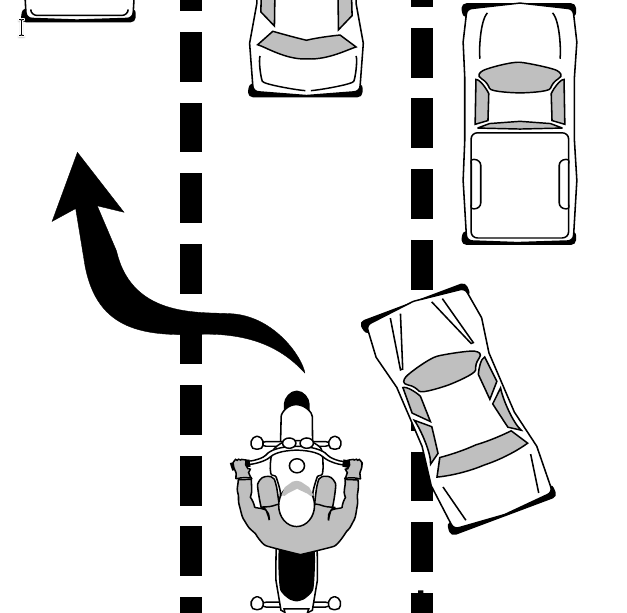
\includegraphics[width=0.95\textwidth, frame]{images/swerve_then_brake.png}
		\caption{Swerve, then brake}
		\label{fig:swerve_then_brake}
	\end{subfigure}
	\hspace*{\fill}
	\begin{subfigure}{0.45\textwidth}	
		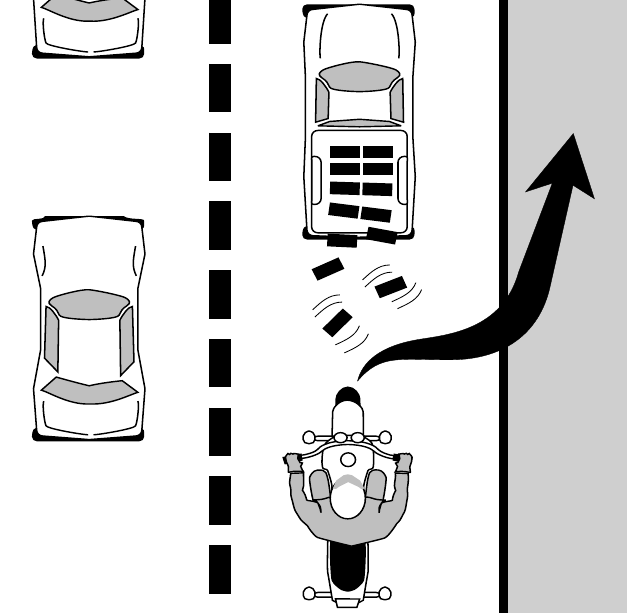
\includegraphics[width=0.95\textwidth, frame]{images/brake_then_swerve.png}
		\caption{Brake, then swerve}
		\label{fig:brake_then_swerve}
	\end{subfigure}
	\caption{Swerving or Turning}
\end{figure}




\begin{langblock}{0.425}
	\begin{eng}
	
	Sometimes you may not have enough room to stop, even if you use both brakes properly. An object might appear suddenly in your path. Or the car ahead might squeal to a stop. The only way to avoid a crash may be to turn quickly, or swerve around it.
	
	A swerve is any sudden change in direction. It can be two quick turns, or a rapid shift to the side. Apply a small amount of pressure to the handgrip located on the side of your intended direction of escape. This will cause the motorcycle to lean quickly. The sharper the turn(s), the more the motorcycle must lean.
	
	Keep your body upright and allow the motorcycle to lean in the direction of the turn while keeping your knees against the tank and your feet solidly on the pegs. Let the motorcycle move underneath you. Make your escape route the target of your vision. Press on the opposite handgrip once you clear the obstacle to return you to your original direction of travel. To swerve to the left, press the left handgrip, then press the right to recover. To swerve to the right, press right, then left.
	
	
	IF BRAKING IS REQUIRED, SEPARATE IT FROM SWERVING.  Brake before or after -- never while swerving.
	\end{eng}
	\begin{rus}
		
		Даже если вы правильно используете оба тормоза, у вас может не хватить места для остановки. 
%		На вашем пути может внезапно появиться препятствие. Или автомобиль впереди может резко затормозить. 
		И тогда единственный способ избежать столкновения "--- быстрый поворот или маневр уклонения.
		
		Маневр уклонения -- это любое резкое изменение направления движения. Это могут быть два быстрых поворота или резкое смещение в сторону. Слегка нажмите на ручку, расположенную со стороны предполагаемого направления маневра. Это заставит мотоцикл быстро наклониться. Чем резче поворот, тем сильнее должен наклониться мотоцикл.
		
		Держите тело в вертикальном положении, а мотоциклу позвольте наклониться в сторону поворота, при этом прижимая колени к баку и крепко удерживая ноги на подножках. Позвольте мотоциклу двигаться под вами. Взгляд на маршруте маневра, а не на препятствии. Как только вы объедите препятствие, нажмите на ручку противоположной стороны, чтобы вернуться к исходному направлению движения. Чтобы свернуть влево, нажмите на левую ручку, а затем на правую, чтобы восстановить направление. Чтобы свернуть вправо, нажмите на правую ручку, а затем на левую.\footnote{В отличии от обычного поворота, где Вы и мотоцикл наклоняются вместе, в случае резкого маневр уклонения на это нет времени, потому тело должно оставаться вертикально, а байк извивается обходя препятствие.}
		
		
		ЕСЛИ ТРЕБУЕТСЯ ТОРМОЖЕНИЕ, ДЕЛАЙТЕ ЭТО ОТДЕЛЬНО ОТ МАНЕВРИРОВАНИЯ.  Тормозите до или после, но не во время маневра.
\end{rus}
\end{langblock}








\langsection[subsubsection]{Cornering}{Прохождение поворотов}


\begin{figure}[htbp]
	\begin{subfigure}{0.45\textwidth}
		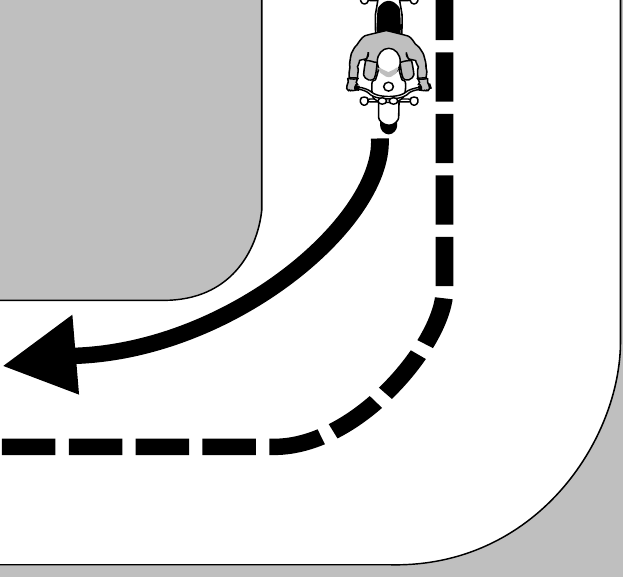
\includegraphics[width=0.95\textwidth, frame]{images/curve_const.png}
		\caption{Constant curves}
		\label{fig:curve_const}
	\end{subfigure}
	\hspace*{\fill}
	\begin{subfigure}{0.45\textwidth}
		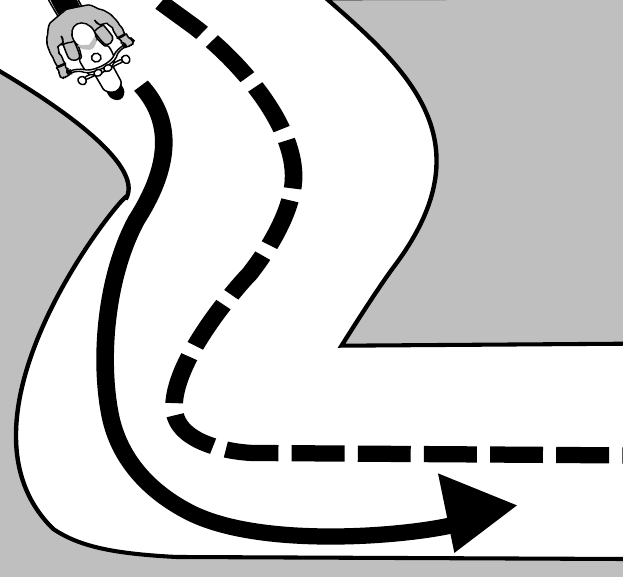
\includegraphics[width=0.95\textwidth, frame]{images/curve_multi.png}
		\caption{Multiple curves}
		\label{fig:curve_multi}
	\end{subfigure}
	
	\begin{subfigure}{0.45\textwidth}
		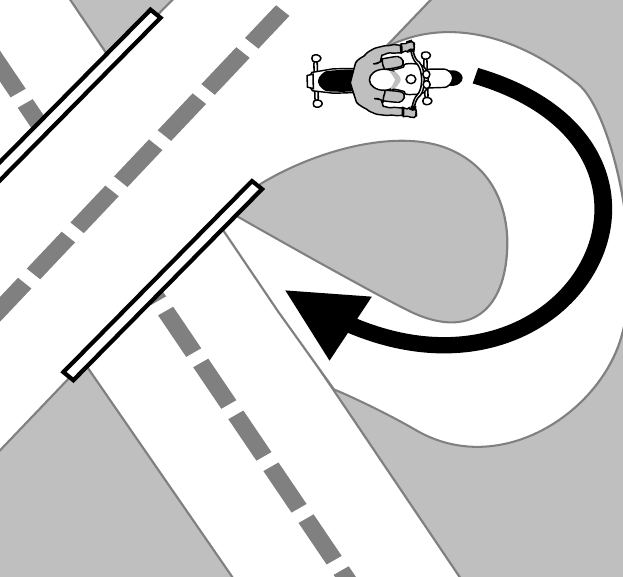
\includegraphics[width=0.95\textwidth, frame]{images/curve_decr.png}
		\caption{Decreasing curves}
		\label{fig:curve_decr}
	\end{subfigure}
	\hspace*{\fill}
	\begin{subfigure}{0.45\textwidth}
		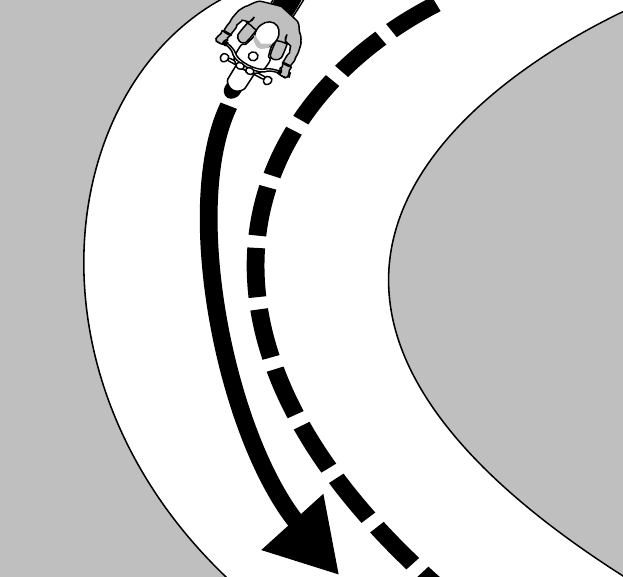
\includegraphics[width=0.95\textwidth, frame]{images/curve_widening.png}
		\caption{Widening curves}
		\label{fig:curve_widening}
	\end{subfigure}
	
	\caption{Cornering}
\end{figure}

\begin{langblock}{0.425}
	\begin{eng}
	
	A primary cause of single-vehicle crashes is motorcyclists running wide in a curve or turn and colliding with the roadway or a fixed object.
	
	Every curve is different. Be alert to whether a curve remains constant, gradually widens, gets tighter, or involves multiple turns.
	
	Ride within your skill level and posted speed limits.
	
	Your best path may not always follow the curve of the road. Change lane position depending on traffic, road conditions and curve of the road.  If no traffic is present, start at the outside of a curve to increase your line of sight and the effective radius of the turn. As you turn, move toward the inside of the curve, and as you pass the center, move to the outside to exit.
	
	Another alternative is to move to the center of your lane before entering a curve -- and stay there until you exit. This permits you to spot approaching traffic as soon as possible. You can also adjust for traffic crowding the center line, or debris blocking part of your lane.
	\end{eng}
	\begin{rus}
		
		Одной из основных причин ДТП без участия других транспортных средств: выезд за пределы полосы в повороте, наезд на элементы дороги или неподвижный объект (обочина, кювет, отбойник, столб, опора).
		
		Каждый поворот уникален. Следите за тем, остается ли радиус поворота постоянным, растет, уменьшается или состоит из нескольких виражей.
		
		Езжайте в пределах своих навыков и соблюдайте установленные ограничения скорости.
		
		Оптимальная траектория движения не всегда совпадает с кривизной полосы и разметки. Меняйте положение в полосе движения в зависимости от интенсивности движения других участников, состояния дороги и кривизны поворота. Если вы на дороге один, начинайте поворот с внешней стороны, чтобы увеличить обзор и эффективный радиус поворота. По мере прохождения поворота смещайтесь к внутренней стороне, а после прохождения центра поворота "--- к внешней, чтобы выехать из поворота.\footnote{Техника распрямления поворота, увеличение радиуса. Но она не должна пониматься слишком буквально. На входе в поворот внешняя сторона, затем на пике поворота внутренняя, и на выходе снова внешняя. Но это не значит, что надо касаться или наезжать на разметку. На внешних краях мусор и песок, а на внутренней "--- встречный транспорт, который часто срезает излишние изгибы.}
		
		Другой вариант "--- не понтоваться, перед входом в поворот сбросить скорость, переместиться в центр своей полосы движения и оставаться там до выхода из поворота. Это позволит вам как можно раньше заметить приближающийся транспорт. Вы также сможете скорректировать траекторию в случае, если другой транспорт «претендует» на центральную часть или на вашей полосе окажутся препятствия.
\end{rus}
\end{langblock}













